\begin{tikzpicture}
  \node[anchor=south west, inner sep=0] (image) at (0, 0) {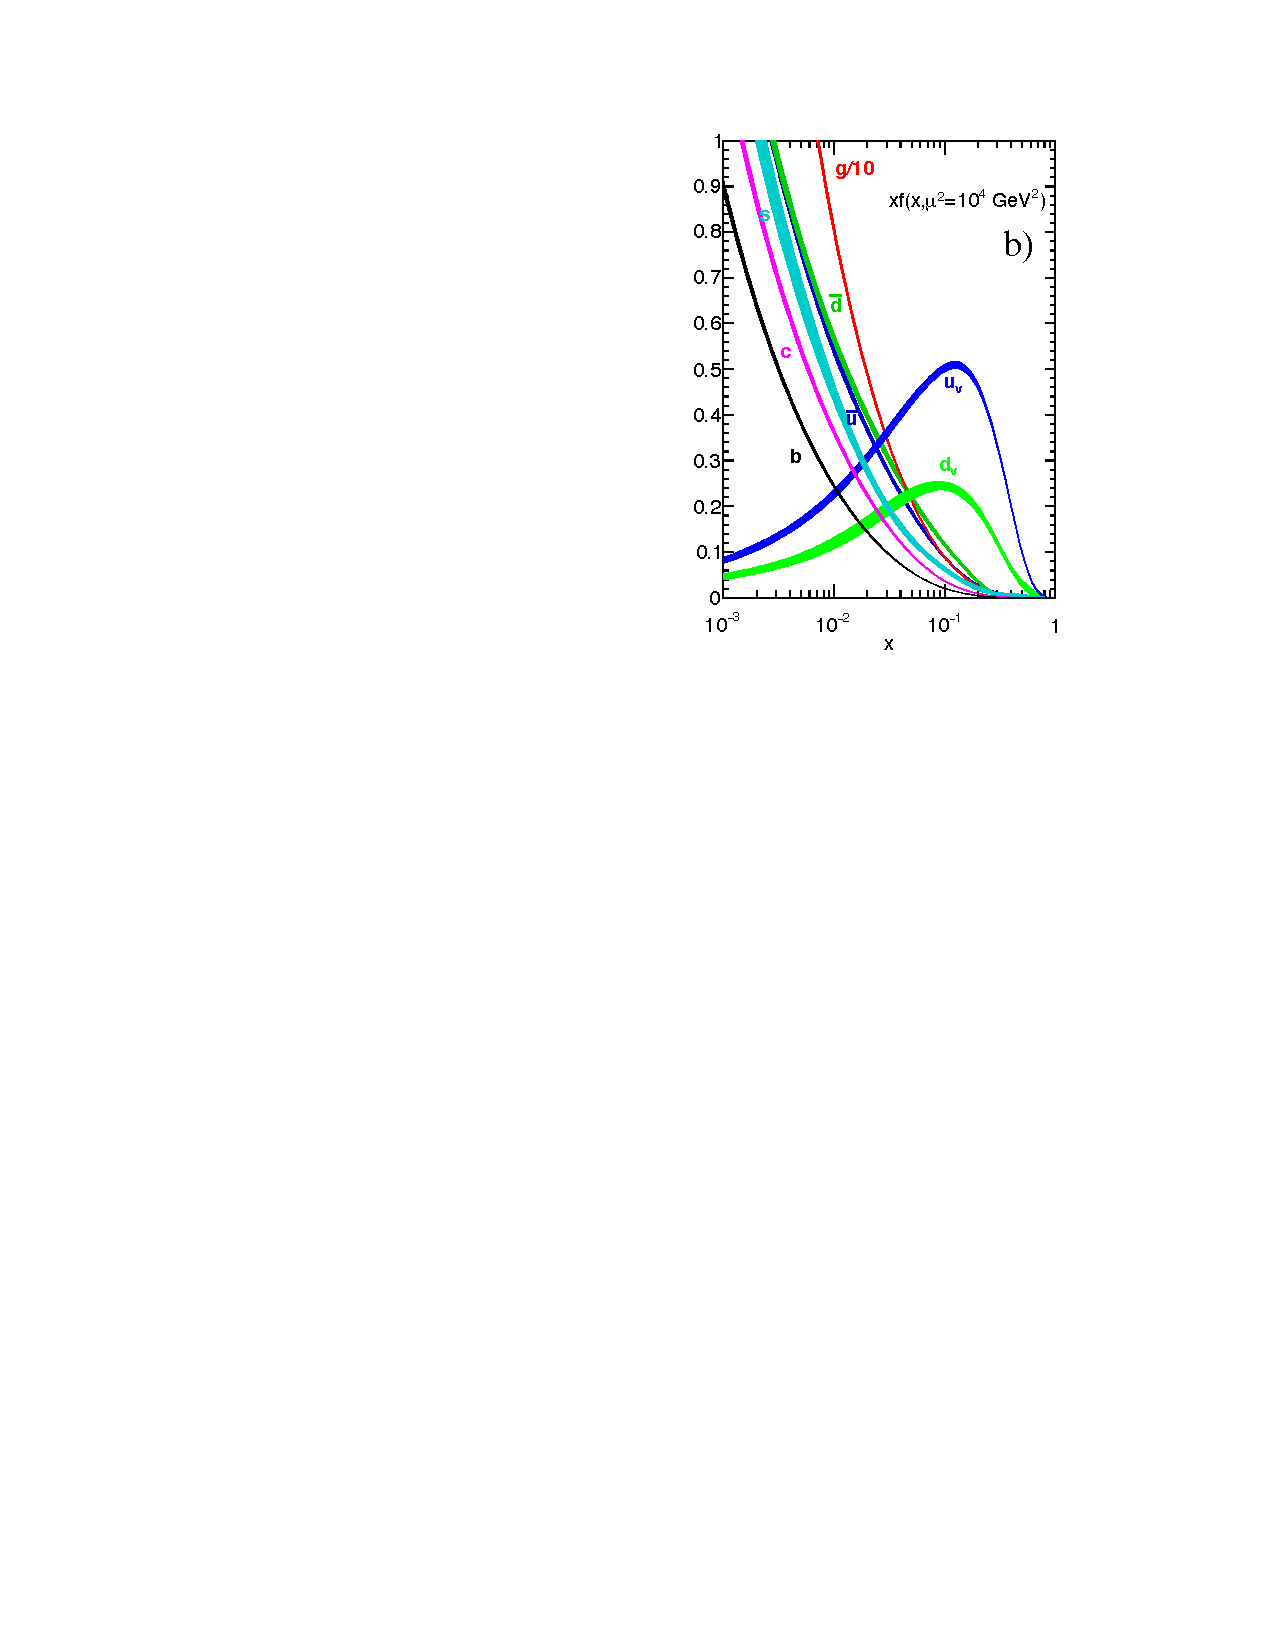
\includegraphics[width=\textwidth]{figures/production/pdf_sets_high_qsquared}};
  \begin{scope}[x={(image.south east)}, y={(image.north west)}]
    % Grid to help find coordinates on the image
    % \draw[step=0.02, gray, very thin] (0, 0) grid (1, 1);
    % Box to cover 'b)' label
    \path[fill=white] (0.82, 0.74) rectangle (0.94, 0.82);
  \end{scope}
\end{tikzpicture}
